\input{preamble-slides169}

%Tick mark commands
\newcommand\ticks{}
  \def\ticks{{Bar[scale=2]}-{Bar[scale=2]}}
\newcommand\paraticks{}
  \def\paraticks{{Straight Barb[reversed, scale=2]}-{Straight Barb[scale=2]}}

\title{Geometry Unit 9: Dilation and similarity}
\date{13 March 2023 - 31 March 2023}

\begin{document}
\frame{\titlepage}
\section[Outline]{}
\frame{\tableofcontents}

\section{9.1 Dilation introduction \hfill 13 March \,}
\begin{frame}{Learning Target: I can dilate a triangle}
  {HSG.SRT.B.5 Use similarity criteria for triangles to solve problems \hfill \alert{9.1 Monday 13 March}}
    Do Now
    \begin{enumerate}
      \item $12 \times \frac{1}{3}=$
      \item $10 \times \frac{7}{5}=$
      \item Find $x$ if $9 \cdot x = 15$
    \end{enumerate}
    Lesson: Dilation, transformations, fraction operations \\
    Test results, check Jumprope\\[0.5cm]
    Homework: Complete the classwork practice, Deltamath problem set
\end{frame}

\begin{frame}{Dilation, similarity, and scaled proportions}
  {Write this information in your notebook}
  \begin{columns}
    \column{0.6\textwidth}
      \begin{description}
        \item[Similarity] Objects with the same shape, but not necessarily the same size, are similar. Their corresponding angles are congruent and their corresponding sides are proportional.
        \item[Notation] This is the symbol for similar triangles: $\triangle ABC \sim \triangle DEF$
        \item[Dilation] A transformation that stretches objects on the plane by a factor away from a point
        \item[Scale factor] The ratio of the lengths of the corresponding sides of dilated figures
        \item[Definition] Two figures are similar if one or more rigid motions and a dilation will carry one figure onto the other.
      \end{description}
    \column{0.4\textwidth}
    \begin{flushright}
      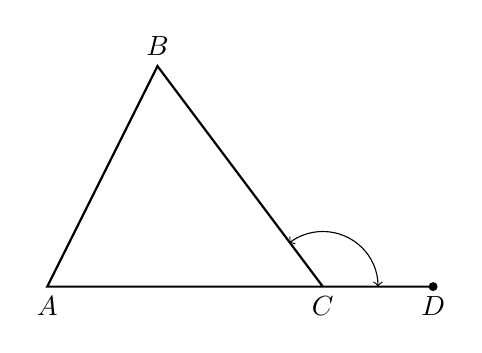
\begin{tikzpicture}[scale=0.7]
        \draw [thick]
        (9,0)node[below]{$D$}--
        (2,0)node[below]{$A$}--
        (4,4)node[above]{$B$}--
        (7,0)node[below]{$C$};
        \draw [fill] (9,0) circle [radius=0.07];
        \draw[<->] (8,0) arc (0:128:1);
        %\node at (2.8,0.4){$52^\circ$};
        %\node at (4.1,3.1){$48^\circ$};
      \end{tikzpicture}
    \end{flushright}
  \end{columns}
\end{frame}

\section{8.3 Midpoint, segment partition \hfill 16 February \,}
\begin{frame}{Learning Target: I can partition a line segment}
  {HSG.GPE.B.6 Partition a segment in a given ratio \hfill \alert{8.3 Thursday 16 February}}
  \begin{columns}
    \column{0.5\textwidth}
    Do Now: \\Given $T_{+a,+b}$ maps $(3,5) \rightarrow (9,8)$ \\
    Find $a$ and $b$ \\[0.5cm]
    Lesson: Ratios, partitioning a line segment \\
    Homework: Complete classwork, Deltamath assignment
    \column{0.4\textwidth}
    \begin{flushright}
      \begin{tikzpicture}[scale=0.5]
        \draw[thick, <->] (-1.4,0) -- (9.4,0) node [below right] {$x$};
        \draw[thick, <->] (0,-1.4)--(0,8.4) node [left] {$y$};
        \draw[thick, ->] (3,5)--(8.8,7.9);
        \draw [fill] (3,5) circle [radius=0.1] node[below right] {$A(3,5)$};
        \draw [fill] (9,8) circle [radius=0.1] node[above left] {$B(9,8)$};
      \end{tikzpicture}
    \end{flushright}
  \end{columns}
\end{frame}

\section{8.5 Analytic geometry graphing \hfill 3 March \,}
\begin{frame}{Learning Target: I can graph linear equations and systems}
  {HSA.REI.C.6 Solve systems of linear equations \hfill \alert{8.5 Friday 3 March}}
  \begin{columns}
    \column{0.6\textwidth}
    Do Now: Graph the line $y=\frac{1}{2}x+2$ \\[0.5cm]
    Lesson: slope-intercept form, systems \\
    Homework: Complete classwork, Deltamath assignment
    \column{0.4\textwidth}
    \begin{flushright}
      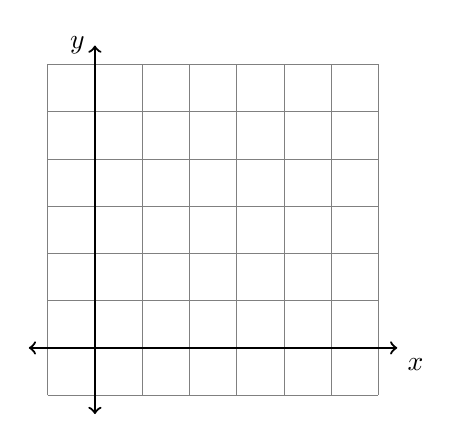
\begin{tikzpicture}[scale=0.6]
        \draw[help lines] (-1,-1) grid (6,6);
        \draw[thick, <->] (-1.4,0) -- (6.4,0) node [below right] {$x$};
        \draw[thick, <->] (0,-1.4)--(0,6.4) node [left] {$y$};
      \end{tikzpicture}
    \end{flushright}
  \end{columns}
\end{frame}

\begin{frame}{Solving a system using a graphing calculator}
  \begin{columns}
    \column{0.6\textwidth}
    $$f(x)=-\frac{1}{2}x+6$$
    $$g(x)=\frac{3}{4}x+1$$
      \onslide<2->{$f(4)=-\frac{1}{2}(4)+6=-2+6=4$ \\
      $g(4)=\frac{3}{4}(4)+1=3+6=4$}
    \onslide<1>{\begin{description}
      \item[system] two or more equations with the same variables
      \item[intersection] the point where two lines cross, or the $(x,y)$ values that satisfy both equations
    \end{description}}
    \column{0.4\textwidth}
    \begin{flushright}
      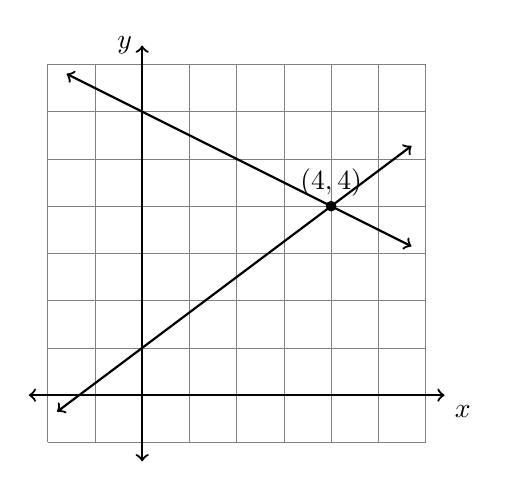
\begin{tikzpicture}[scale=0.6]
        \draw[help lines] (-2,-1) grid (6,7);
        \draw[thick, <->] (-2.4,0) -- (6.4,0) node [below right] {$x$};
        \draw[thick, <->] (0,-1.4)--(0,7.4) node [left] {$y$};
        \pause
          \draw[thick, <->,domain=-1.6:5.7] plot(\x,-0.5*\x+6);
          \draw[thick, <->,domain=-1.8:5.7] plot(\x,0.75*\x+1);
          \draw [fill] (4,4) circle [radius=0.1]node[above]{$(4,4)$};
      \end{tikzpicture}
    \end{flushright}
  \end{columns}
\end{frame}

\section{8.6 Analytic geometry slope applications \hfill 6 March \,}
\begin{frame}{Learning Target: I can use slope to solve problems}
  {HSG.GPE.B.5 Use slope to solve geometric problems \hfill \alert{8.6 Monday 6 March}}
  \begin{columns}
    \column{0.6\textwidth}
    Do Now: Solve the system in your graphing calculator: 
      $$f(x)=-x+2$$
      $$g(x)=-3x-2$$
    \onslide<1>{
      Lesson: Perpendicular and parallel slopes, applications \\
      Homework: Complete classwork, Deltamath assignment}
    \column{0.4\textwidth}
    \begin{flushright}
      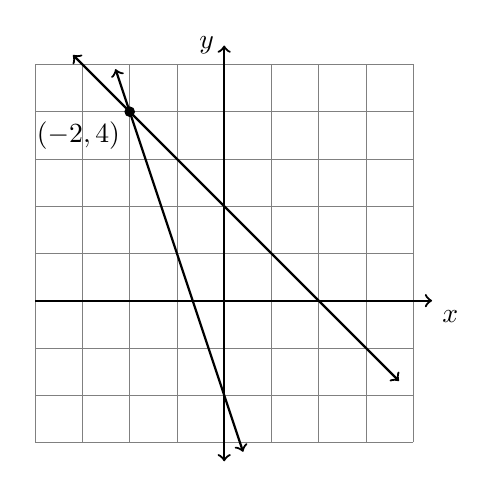
\begin{tikzpicture}[scale=0.6]
        \draw[help lines] (-4,-3) grid (4,5);
        \draw[thick, ->] (-4,0) -- (4.4,0) node [below right] {$x$};
        \draw[thick, <->] (0,-3.4)--(0,5.4) node [left] {$y$};
        \pause
          \draw[thick, <->,domain=-3.2:3.7] plot(\x,-\x+2);
          \draw[thick, <->,domain=-2.3:0.4] plot(\x,-3*\x-2);
          \draw [fill] (-2,4) circle [radius=0.1]node[below left]{$(-2,4)$};
      \end{tikzpicture}
    \end{flushright}
  \end{columns}
\end{frame}

\begin{frame}{Use slopes to prove special polygons}
  \begin{columns}
    \column{0.6\textwidth}
    Find each line's equation and their relationships
    \begin{enumerate}
      \item Find the equation of line $f$
      \item Find the equation of line $k$
      \item Show that $f \perp k$ because $m_f \times m_k = -1$
      \item Find and label the slopes of $g$ and $l$
      \item Show the polygon is a rectangle
    \end{enumerate}
    \column{0.4\textwidth}
    \begin{flushright}
      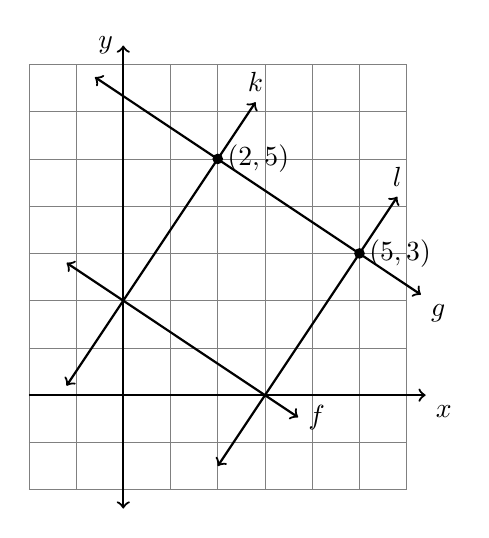
\begin{tikzpicture}[scale=0.6]
        \draw[help lines] (-2,-2) grid (6,7);
        \draw[thick, ->] (-2.0,0) -- (6.4,0) node [below right] {$x$};
        \draw[thick, <->] (0,-2.4)--(0,7.4) node [left] {$y$};
        \draw[thick, <->,domain=-1.2:3.7] plot(\x,-0.667*\x+2)node[right]{$f$};
        \draw[thick, <->,domain=-1.2:2.8] plot(\x,1.5*\x+2)node[above]{$k$};
        \draw[thick, <->,domain=-0.6:6.3] plot(\x,-0.667*\x+6.33)node[below right]{$g$};
        \draw[thick, <->,domain=2:5.8] plot(\x,1.5*\x-4.5)node[above]{$l$};
        \draw [fill] (2,5) circle [radius=0.1]node[right]{$(2,5)$};
        \draw [fill] (5,3) circle [radius=0.1]node[right]{$(5,3)$};
      \end{tikzpicture}
    \end{flushright}
  \end{columns}
\end{frame}

\section{8.7 Analytic geometry distance applications \hfill 7 March \,}
\begin{frame}{Learning Target: I can calculate distance in context}
  {HSG.GPE.B.7 Use coordinates to compute perimeters of polygons \hfill \alert{8.7 Tuesday 7 March}}
  \begin{columns}
    \column{0.6\textwidth}
    Do Now: Find the distance between the intercepts of the line show on the graph \\[0.5cm]
    Lesson: Distance formula, applications, simplifying radicals \\
    Homework: Complete classwork, Deltamath assignment \\[0.5cm]
    \alert{Unit test Friday}, Deltamath and problem sets due
    \column{0.4\textwidth}
    \begin{flushright}
      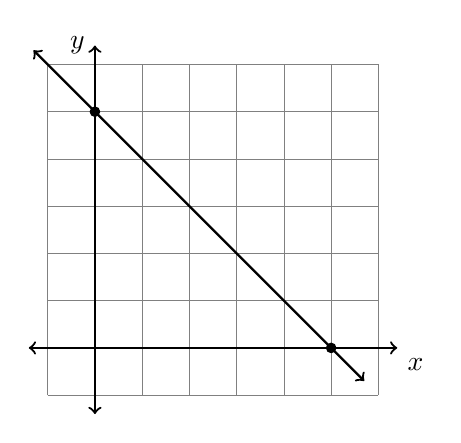
\begin{tikzpicture}[scale=0.6]
        \draw[help lines] (-1,-1) grid (6,6);
        \draw[thick, <->] (-1.4,0) -- (6.4,0) node [below right] {$x$};
        \draw[thick, <->] (0,-1.4)--(0,6.4) node [left] {$y$};
        \draw[thick, <->,domain=-1.3:5.7] plot(\x,-1*\x+5);
        \draw [fill] (5,0) circle [radius=0.1];
        \draw [fill] (0,5) circle [radius=0.1];
      \end{tikzpicture}
    \end{flushright}
  \end{columns}
\end{frame}

\begin{frame}{Use distance to prove special polygons}
  \begin{columns}
    \column{0.6\textwidth}
    Prove the quadrilateral is a rhombus
    \begin{enumerate}
      \item Apply the distance formula to each pair of points
      \item State the equality of the side lengths and the congruence of the sides
      \item State the conclusion, that the quadrilateral is a rhombus
    \end{enumerate}
    \column{0.4\textwidth}
    \begin{flushright}
      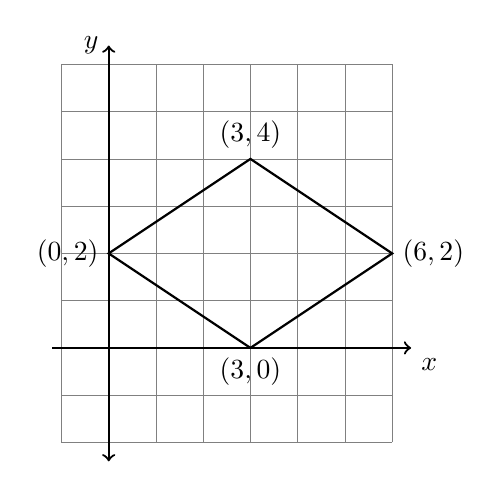
\begin{tikzpicture}[scale=0.6]
        \draw[help lines] (-1,-2) grid (6,6);
        \draw[thick, ->] (-1.2,0) -- (6.4,0) node [below right] {$x$};
        \draw[thick, <->] (0,-2.4)--(0,6.4) node [left] {$y$};
        \draw[thick] (0,2)node[left]{$(0,2)$}--
          (3,4)node[above]{$(3,4)$}--
          (6,2)node[right]{$(6,2)$}--
          (3,0)node[below]{$(3,0)$} -- cycle;
      \end{tikzpicture}
    \end{flushright}
  \end{columns}
\end{frame}

\section{8.8 Peer unit review \hfill 9 March \,}
\begin{frame}{Learning Target: I can use volume formulas to solve problems}
  {HSG.GMD.A.3 Use volume formulas to solve problems \hfill \alert{8.8 Thursday 9 March}}
    Do Now: Write in your notebook
    \begin{enumerate}
      \item Your strongest two skills in this unit
      \item Your weakest 2 topics (and why)
      \item Your current Jumprope grade
      \item Your goal for this trimester's report card grade in Geometry
    \end{enumerate} \bigskip
    Lesson: Unit review \\
    Notebook check, uniforms professionalism grade \\[0.5cm]
    \alert{Unit test tomorrow}, Deltamath and problem sets due
\end{frame}

\begin{frame}{Notebook check scoring}
  {Start quickly at the beginning of class: notebook, pencil, folder, calculator; get to work}
    Jumprope mastery score
    \begin{enumerate}
      \item I have a notebook $\rightarrow$ 1
      \item I have class notes $\rightarrow$ 2
      \item I have stars indicating I quickly sit down and write the learning target $\rightarrow$ 3
      \item I have stars and I complete the Do Now right away $\rightarrow$ 4
    \end{enumerate} \bigskip
\end{frame}

\end{document}